\documentclass[11pt]{article}

\usepackage[a4paper,margin=1in]{geometry}
\usepackage{graphicx}
\usepackage{booktabs}
\usepackage{xcolor}
\usepackage{hyperref}
\usepackage{listings}
\usepackage{subcaption}

\hypersetup{
  colorlinks=true,
  linkcolor=blue!55!black,
  urlcolor=blue!55!black,
  citecolor=blue!55!black
}

\lstdefinestyle{python}{
  language=Python,
  basicstyle=\ttfamily\small,
  keywordstyle=\color{blue!60!black},
  commentstyle=\color{green!40!black},
  stringstyle=\color{red!50!black},
  showstringspaces=false,
  breaklines=true,
  frame=single,
  rulecolor=\color{black!20},
  tabsize=2
}

\title{LISA Link Simulation: Waveform to Six Links and TDI}
\author{LISA-TF simulation notes}
\date{\today}

\begin{document}
\maketitle

\begin{abstract}
This note documents the simulation part of the repository: a user-provided
gravitational-wave strain waveform is placed on a science time grid, propagated
through a realistic LISA orbit to form six one-way link responses, injected into
\texttt{lisainstrument} noise, and converted to Michelson \texttt{XYZ} and
orthogonal \texttt{AET} TDI products with \texttt{PyTDI}. The diagnostic figures
come from the MBHB run in \path{diagnostics/mbhb_sixlinks}.
\end{abstract}

\section{Scope}

The reusable entry point is \path{scripts/lisa_link_simulation.py}. It exposes a
small facade around three pieces of code:
\begin{itemize}
  \item \path{scripts/six_link_generation.py}: waveform preparation, orbit file,
  GW link response, and \texttt{lisainstrument} HDF5 generation.
  \item \path{scripts/tdi_computation.py}: \texttt{XYZ} and \texttt{AET} TDI from
  the full instrument HDF5 and from the GW-only HDF5.
  \item \path{scripts/plotting_utils.py}: diagnostic plots.
\end{itemize}

The simulation is intentionally time-domain until TDI products are optionally
frequency-cut. It writes both science data and provenance files, so later
notebooks can use the saved CSV/HDF5 outputs without rerunning the expensive
instrument stage.

\section{Pipeline}

\begin{center}
\fbox{\begin{minipage}{0.92\linewidth}
\centering
\texttt{t, hplus, hcross}
$\rightarrow$
science-grid waveform
$\rightarrow$
LISA orbit HDF5
$\rightarrow$
six GW links
$\rightarrow$
\texttt{lisainstrument} HDF5
$\rightarrow$
\texttt{PyTDI} \texttt{XYZ}
$\rightarrow$
\texttt{AET}
\end{minipage}}
\end{center}

\begin{table}[h]
\centering
\scriptsize
\begin{tabular}{p{0.18\linewidth}p{0.36\linewidth}p{0.36\linewidth}}
\toprule
Stage & Main routine & Main output \\
\midrule
Waveform alignment & \texttt{prepare\_science\_waveform} & \path{inputs/waveform_aligned.npz} \\
Orbit generation & \texttt{create\_orbit\_file} & \path{inputs/orbits.h5} \\
GW link response & \texttt{compute\_gw\_links} & \path{outputs/six_links_gw_only.csv}, \path{outputs/gws.h5} \\
Instrument run & \texttt{run\_lisa\_instrument} & \path{outputs/lisa_instrument_output.h5} \\
Noisy TDI & \texttt{compute\_tdi\_from\_instrument} & \path{outputs/tdi_michelson_XYZ_AET.csv} \\
GW-only TDI & \texttt{compute\_tdi\_from\_gws} & \path{outputs/tdi_gw_only_XYZ_AET.csv} \\
\bottomrule
\end{tabular}
\caption{Simulation stages and durable outputs.}
\end{table}

\section{Configuration}

The simulation is configured with \texttt{LisaLinkSimulationConfig}. The current
diagnostic convention is:
\begin{itemize}
  \item time frame: TCB seconds since the LISA epoch;
  \item sky frame: ICRS right ascension and declination;
  \item link labels: \texttt{ij} means receiver \texttt{i}, emitter \texttt{j};
  \item orbit dataset: \texttt{tcb/ltt};
  \item GW dataset: \texttt{tcb};
  \item GW links: dimensionless fractional frequency, with \texttt{\_hz} columns
  produced by multiplying by the optical carrier frequency;
  \item TDI unit: frequency, so noisy and GW-only TDI products are compared in Hz.
\end{itemize}

The burn-in segment is prepended before the science segment. It lets
\texttt{lisainstrument} and \texttt{PyTDI} settle before the saved science data
starts. The orbit is generated longer than the waveform, typically
\texttt{orbit\_duration\_factor = 5}, so the science grid lies safely inside the
orbit validity range without generating an unnecessarily long orbit file.

\begin{lstlisting}[style=python,caption={Minimal configuration pattern.}]
from scripts.lisa_link_simulation import LisaLinkSimulationConfig

config = LisaLinkSimulationConfig(
    dt=0.1,
    science_duration=150_000.0,
    burn_in_seconds=600.0,
    edge_taper_seconds=10_000.0,
    frequency_low_hz=1e-5,
    frequency_high_hz=1e-1,
    orbit_duration_factor=5.0,
    orbit_dataset="tcb/ltt",
    gw_dataset="tcb",
    tdi_generation=2,
    tdi_unit="frequency",
)
\end{lstlisting}

\section{Waveform Placement}

The input waveform is a strictly increasing time array and two strain arrays,
\texttt{hplus} and \texttt{hcross}. If \texttt{center\_waveform\_peak=True}, the
largest strain-amplitude sample is placed in the center of the science segment.
Outside the waveform support, the strain is zero-padded. An optional cosine edge
taper suppresses boundary discontinuities.

\begin{figure}[h]
\centering
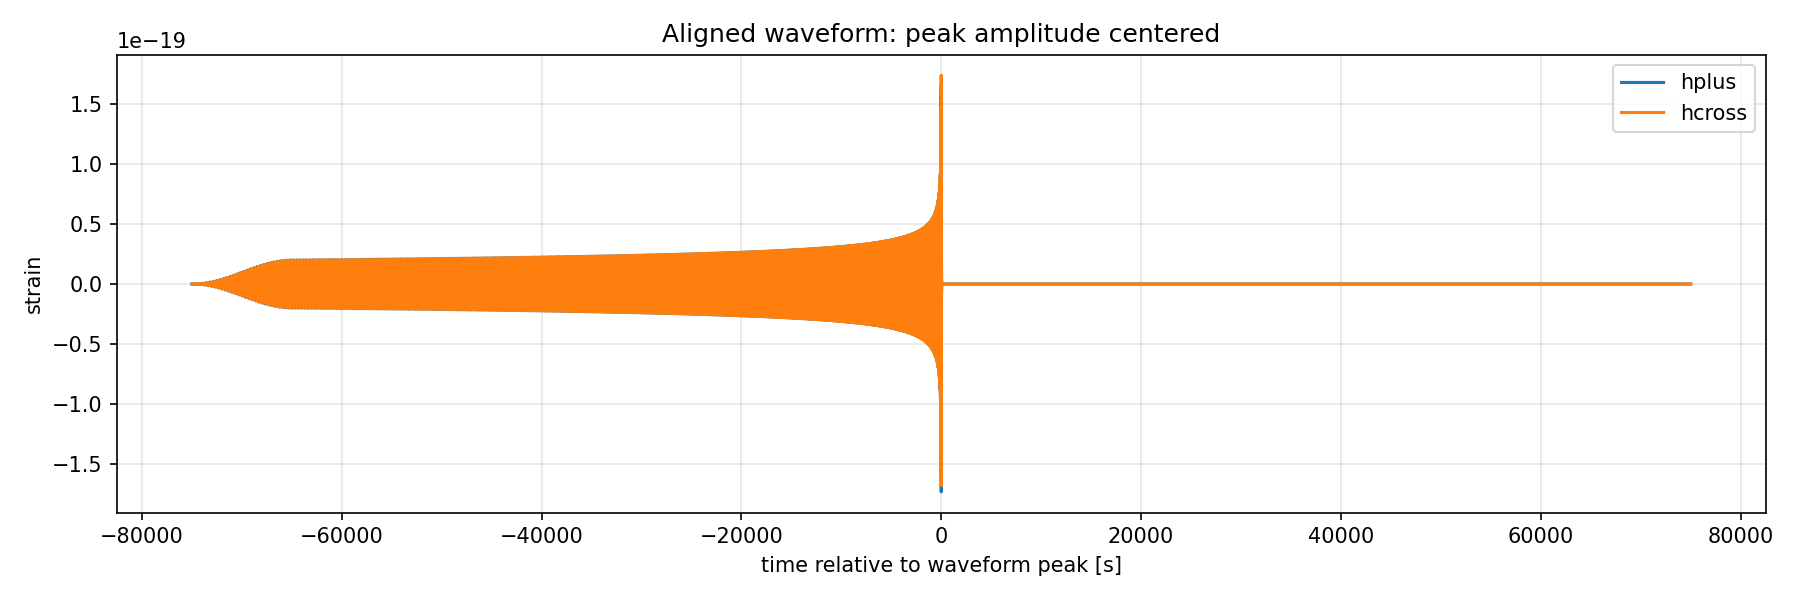
\includegraphics[width=0.92\linewidth]{figures/aligned_waveform.png}
\caption{Prepared MBHB waveform after science-grid placement and edge taper.}
\end{figure}

\section{Six Link Generation}

The six one-way responses are computed with \texttt{lisagwresponse.ReadStrain}
on the LISA orbit time grid. The saved CSV includes both the dimensionless
fractional-frequency link responses and Hz-converted columns:
\[
  y_{ij}^{\mathrm{Hz}}(t) = \nu_0\,y_{ij}(t),
\]
where \(\nu_0 = 2.816\times 10^{14}\,\mathrm{Hz}\) is the optical carrier
frequency used by the instrument simulation.

\begin{figure}[h]
\centering
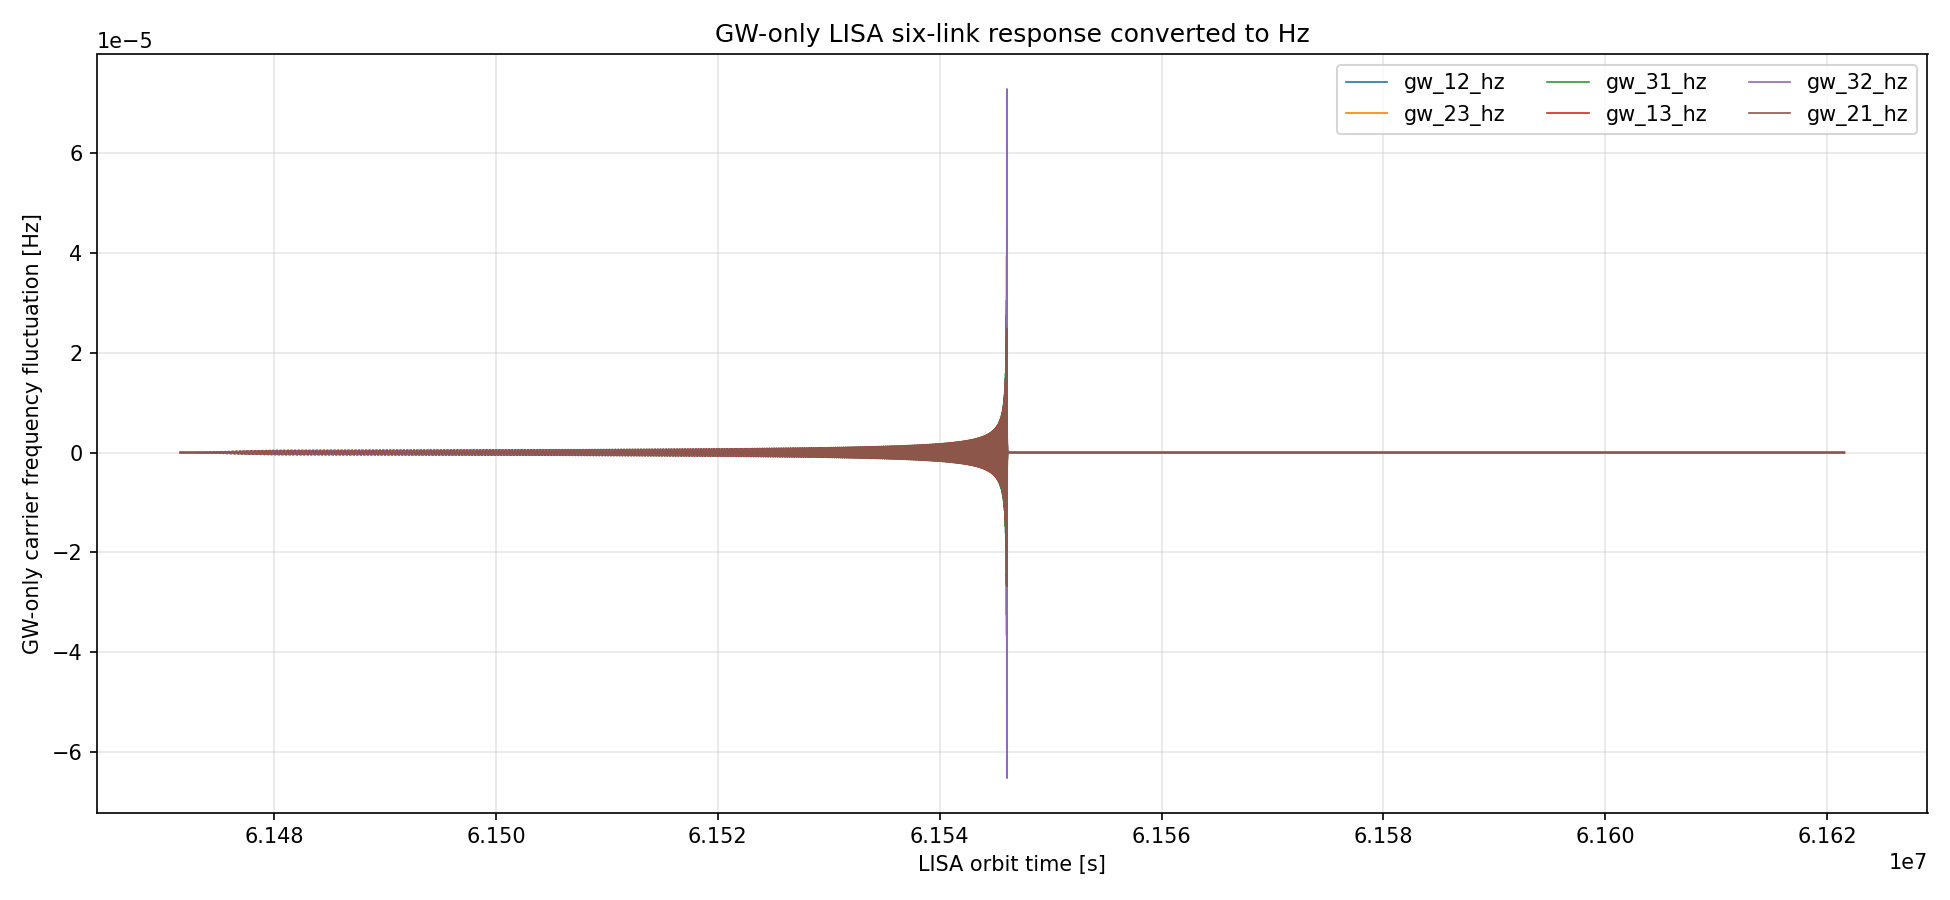
\includegraphics[width=0.92\linewidth]{figures/gw_only_six_links.png}
\caption{GW-only six-link response, converted to Hz for comparison with instrument outputs.}
\end{figure}

\section{Realistic Instrument Noise}

\texttt{lisainstrument.Instrument} reads the orbit HDF5 and the GW HDF5, adds the
instrument noise model, and writes the full measurement HDF5. The exported
\path{six_links_noisy.csv} is a lightweight science-window diagnostic from
\path{debug/sci_carrier_fluctuations}; the realistic TDI products are computed
from the full HDF5 through \texttt{PyTDI}, not only from these debug columns.

\begin{figure}[h]
\centering
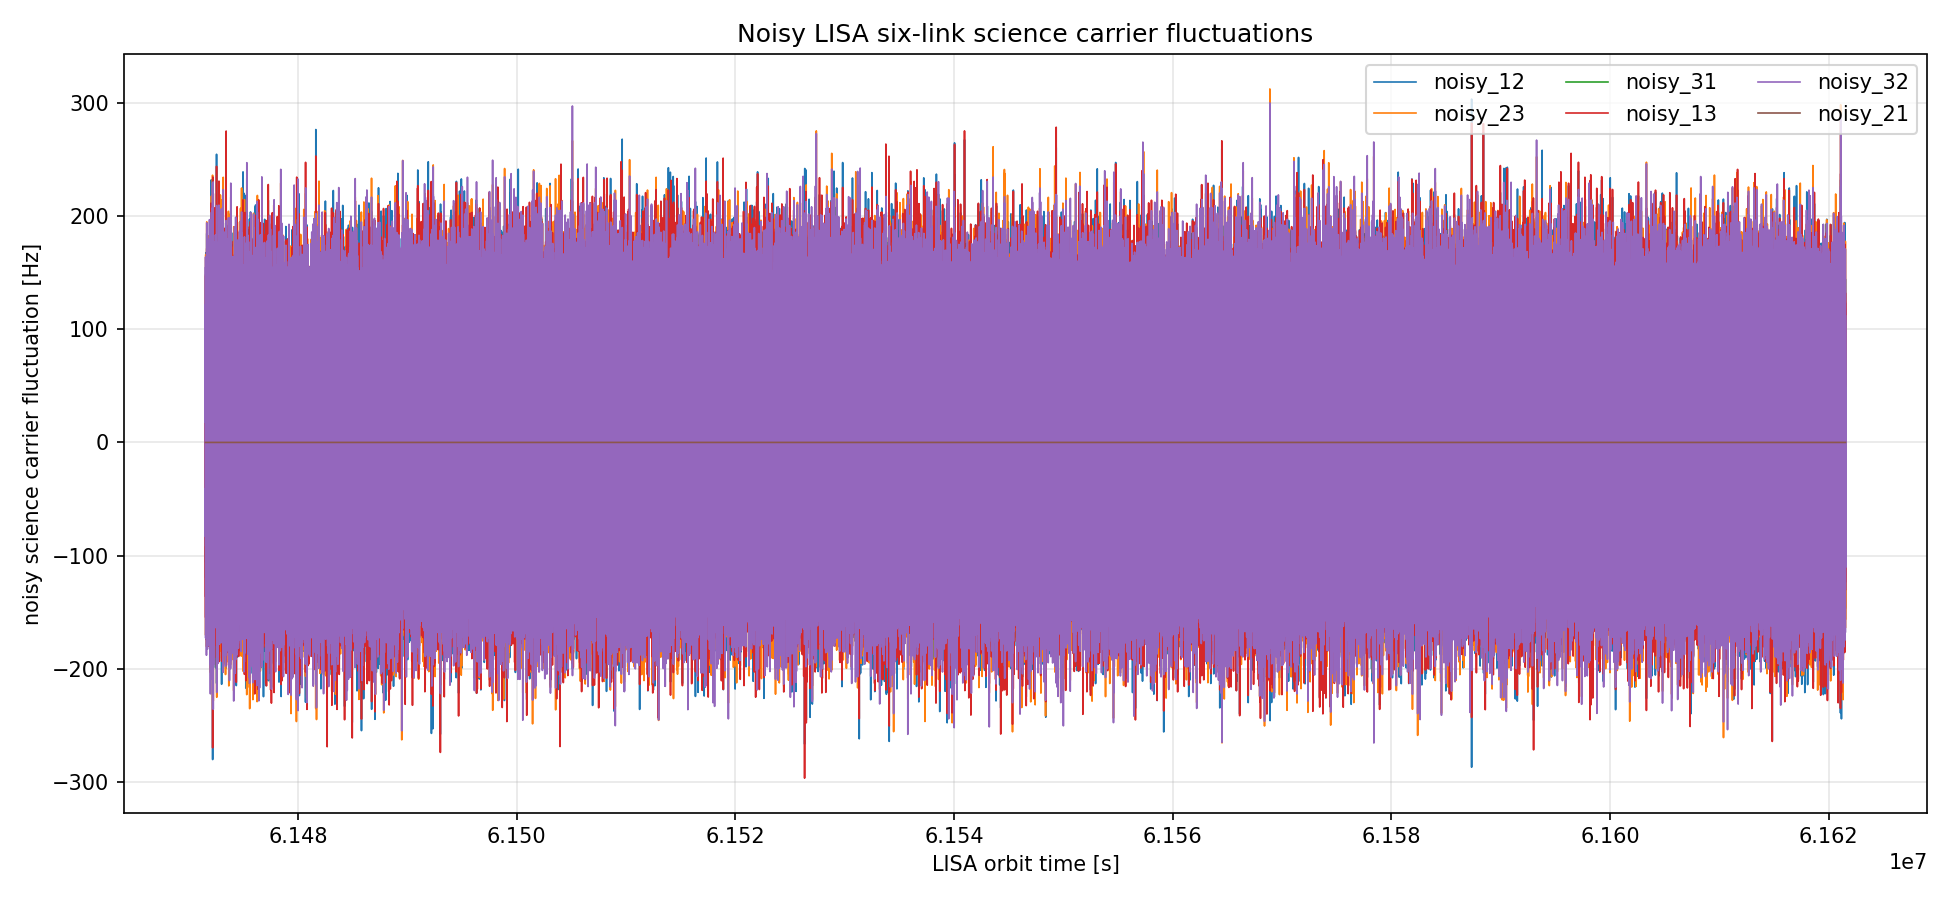
\includegraphics[width=0.92\linewidth]{figures/noisy_six_links.png}
\caption{Science-window noisy link diagnostic from the instrument HDF5.}
\end{figure}

\section{TDI Products}

The noisy TDI path uses
\texttt{Data.from\_instrument(..., signals="fluctuations")} and evaluates
Michelson \texttt{X2}, \texttt{Y2}, and \texttt{Z2}. Orthogonal channels are then
formed as
\[
  A = \frac{Z-X}{\sqrt{2}}, \qquad
  E = \frac{X-2Y+Z}{\sqrt{6}}, \qquad
  T = \frac{X+Y+Z}{\sqrt{3}}.
\]
The GW-only TDI path uses \texttt{Data.from\_gws} and then multiplies by the
same carrier frequency so that the GW-only and noisy TDI products have
consistent units.

The optional frequency cut is applied after TDI in the FFT domain. In the MBHB
diagnostic shown here, the band is \(10^{-5}\) to \(10^{-1}\,\mathrm{Hz}\).

\begin{figure}[h]
\centering
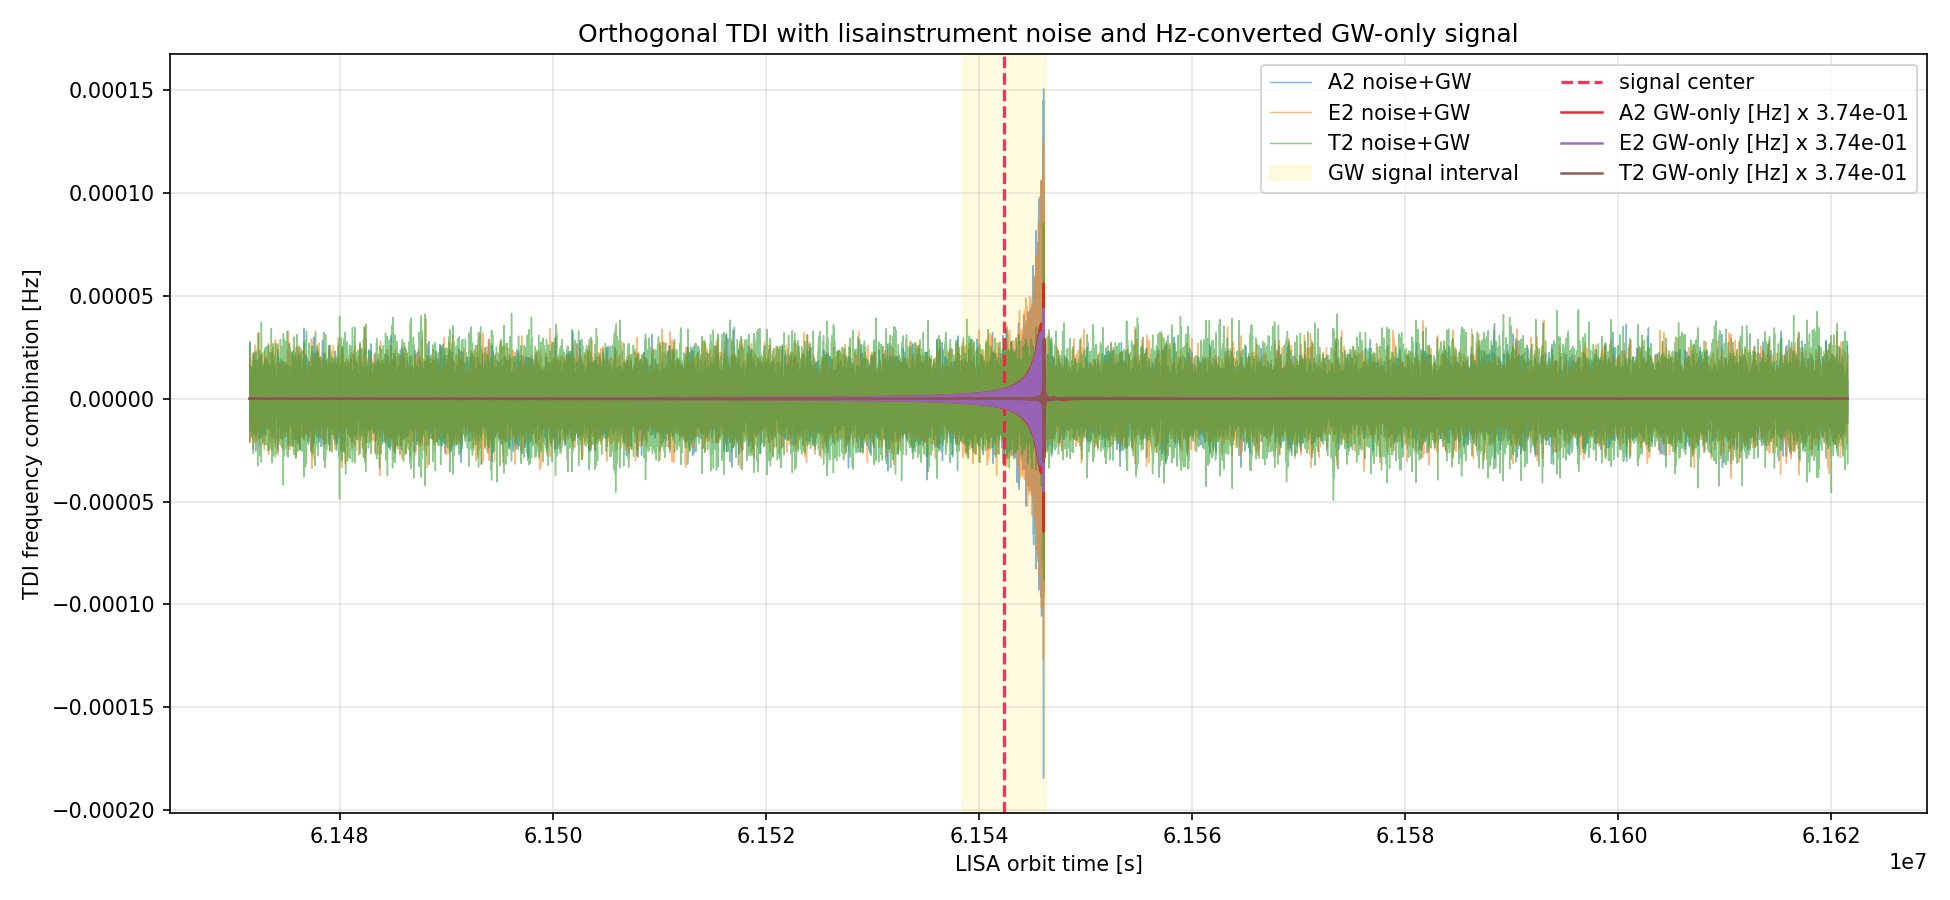
\includegraphics[width=0.92\linewidth]{figures/noisy_aet_with_signal.png}
\caption{Noisy \texttt{AET} TDI with the Hz-converted GW-only signal overlaid for localization in time.}
\end{figure}

\section{Public API}

\begin{lstlisting}[style=python,caption={End-to-end simulation call.}]
from pathlib import Path
from scripts.lisa_link_simulation import (
    LisaLinkSimulationConfig,
    load_npz_waveform,
    run_lisa_link_simulation,
)

t, hplus, hcross = load_npz_waveform("lisa_link_sim/1e5-wave/inputs/my_waveform_1e5.npz")

products = run_lisa_link_simulation(
    t,
    hplus,
    hcross,
    work_dir=Path("examples/runs/minimal_lisa_link_simulation"),
    config=LisaLinkSimulationConfig(),
    make_plots=True,
)
\end{lstlisting}

The returned object contains \texttt{products.paths}, a structured list of all
output paths, and \texttt{products.diagnostics}, scalar checks such as waveform
duration, orbit span, burn-in size, TDI sample count, and signal timing.

\section{SNR Convention}

The SNR diagnostic follows Babak, Hewitson, and Petiteau, \emph{LISA Sensitivity
and SNR Calculations}, LISA-LCST-SGS-TN-001, arXiv:2108.01167. For a
deterministic detector-output/TDI signal \(h\),
\[
  \rho_{\mathrm{opt}} = \sqrt{(h|h)}, \qquad
  (a|b)=4\,\mathrm{Re}\int_0^{f_{\max}}
  \frac{\tilde a^*(f)\tilde b(f)}{S_n(f)}\,df .
\]
Here \(S_n(f)\) is the one-sided PSD of the same TDI channel and in the same
units as the signal. Explicit channels are combined by summing \(\rho_i^2\).

\begin{figure}[h]
\centering
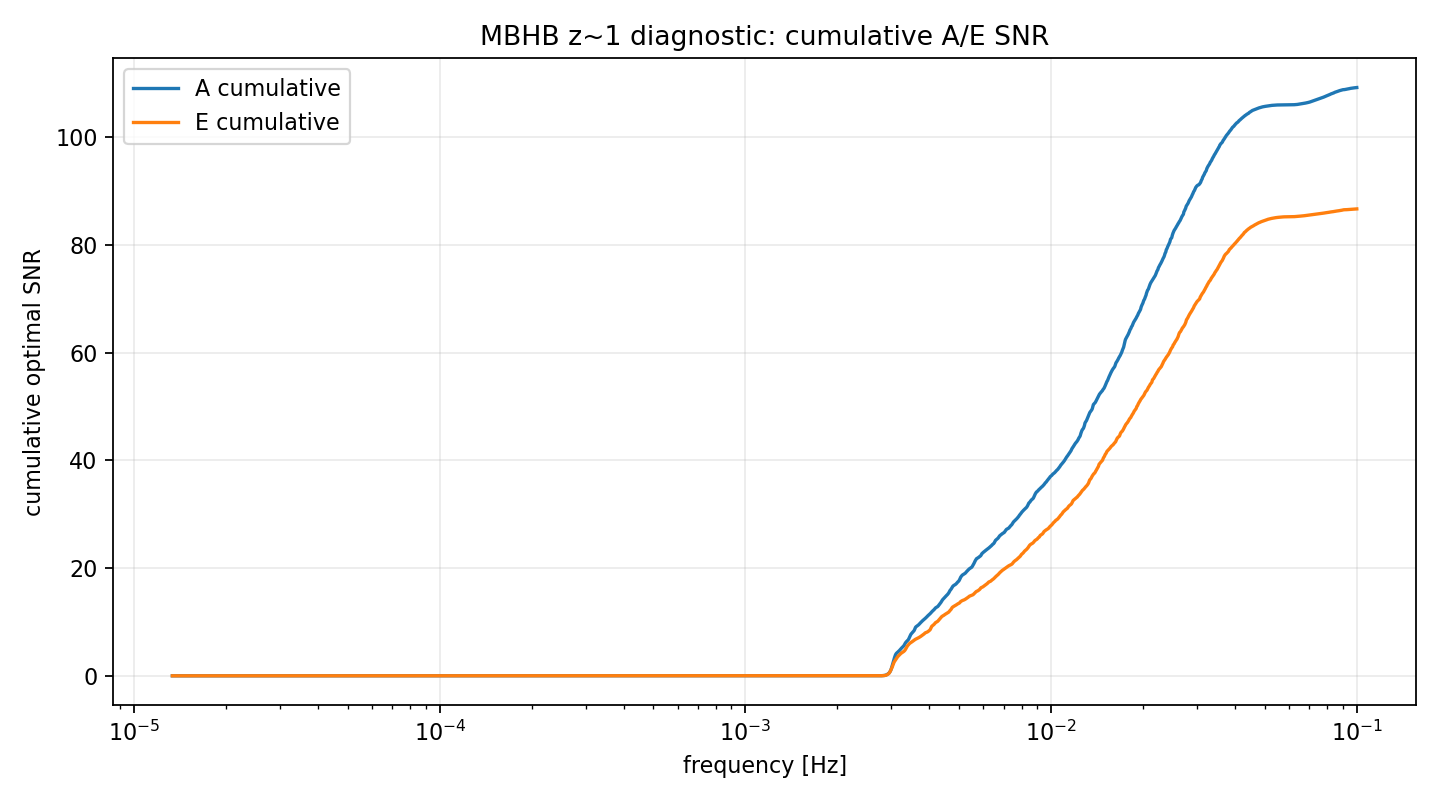
\includegraphics[width=0.82\linewidth]{figures/snr_integrand_ae.png}
\caption{Cumulative \texttt{A/E} optimal SNR for the MBHB diagnostic using the one-sided TDI-channel PSD convention.}
\end{figure}

\section{Minimal Output Contract}

A completed simulation run writes:
\begin{itemize}
  \item \path{six_links_gw_only.csv}: six GW link responses, dimensionless and Hz-converted;
  \item \path{six_links_noisy.csv}: science-window noisy link diagnostic;
  \item \path{tdi_michelson_XYZ_AET.csv}: noisy \texttt{XYZ/AET} TDI in Hz;
  \item \path{tdi_gw_only_XYZ_AET.csv}: GW-only \texttt{XYZ/AET} TDI in Hz;
  \item \path{orbits.h5}, \path{gws.h5}, and \path{lisa_instrument_output.h5}: durable HDF5 provenance.
\end{itemize}

\end{document}
